\documentclass {article}
\usepackage [utf8] {inputenc}
\title {\textbf{4 Selección de las tecnologías}}
\author {Jesús Sánchez Granado}
\usepackage{natbib}
\usepackage{graphicx}
\begin{document}
\maketitle
\begin{itemize}
	\item Node.js: Es un entorno de ejecución asíncrono dirigido por eventos, funciona a base de promesas, es decir, funciones que devolverán un resultado en algún momento del futuro, las promesas se pueden encadenar una tras otra si es que necesitamos los datos producidos por la anterior promesa. Si durante la ejecución de un programa no hay nada que hacer, node.js se “dormirá”. 
	Dado que node no utiliza candados es imposible que se bloqueen los procesos, lo que lo hace bastante adecuado para desarrollar sistemas escalables. Además Daniela ya tenía conocimiento previo de este entorno y es una tecnología que venía impuesta por el proyecto.
	
	\item Angular: Es un framework para la construcción de aplicaciones de página única(SPA a partir de ahora) que utiliza HTML y Typescript. Angular sigue el patrón modelo-vista-controlador, el cual consiste en separar la aplicación en tres partes:
	\begin{itemize}
		\item El modelo: Es la piedra angular del patrón, se encarga de manejar los datos y la lógica de la aplicación.
		\item La vista: Es la parte que se le muestra al usuario.
		\item El controlador: Es la parte que se encarga de comunicar a la vista y al modelo, el controlador recibe el input del usuario a través de la vista y se lo pasa al controlador el cual hace las operaciones necesarias y se lo devuelve al controlador, quien se lo pasa a la vista para mostrárselo al usuario.
	\end{itemize}
	
	
	Angular venía impuesto por el trabajo realizado con anterioridad y, aunque es una tecnología con la que ningún miembro del equipo  estaba familiarizado, es cierto que el diseño de aplicación de página única hace mucho más liviano la ejecución de la aplicación por parte del usuario al no tener unos tiempos de espera tan grandes como los que tendría al cargar de nuevo cada página, lo que la hace una buena elección para un trabajo de esta índole.
	
	\item Gitkraken: Es una herramienta de control de versiones la cual se puede conectar a distintas plataformas de git, haciendo de intermediario entre el usuario y el repositorio de git, el cual en este caso está alojado en github. Hemos escogido esta herramienta para nuestro control de versiones porque permite trabajar desde Windows sin necesidad de saberse los comandos, a diferencia de otras herramientas de control de versiones tiene una representación gráfica muy intuitiva que permite ver la distribución de las ramas, los commits y su evolución, y además permite resolver los conflictos generados al hacer merge dentro de la propia aplicación de una manera bastante sencilla. Esto sumado a la experiencia previa de Victoria con la aplicación ha hecho que sea seleccionada como herramienta de control de versiones.

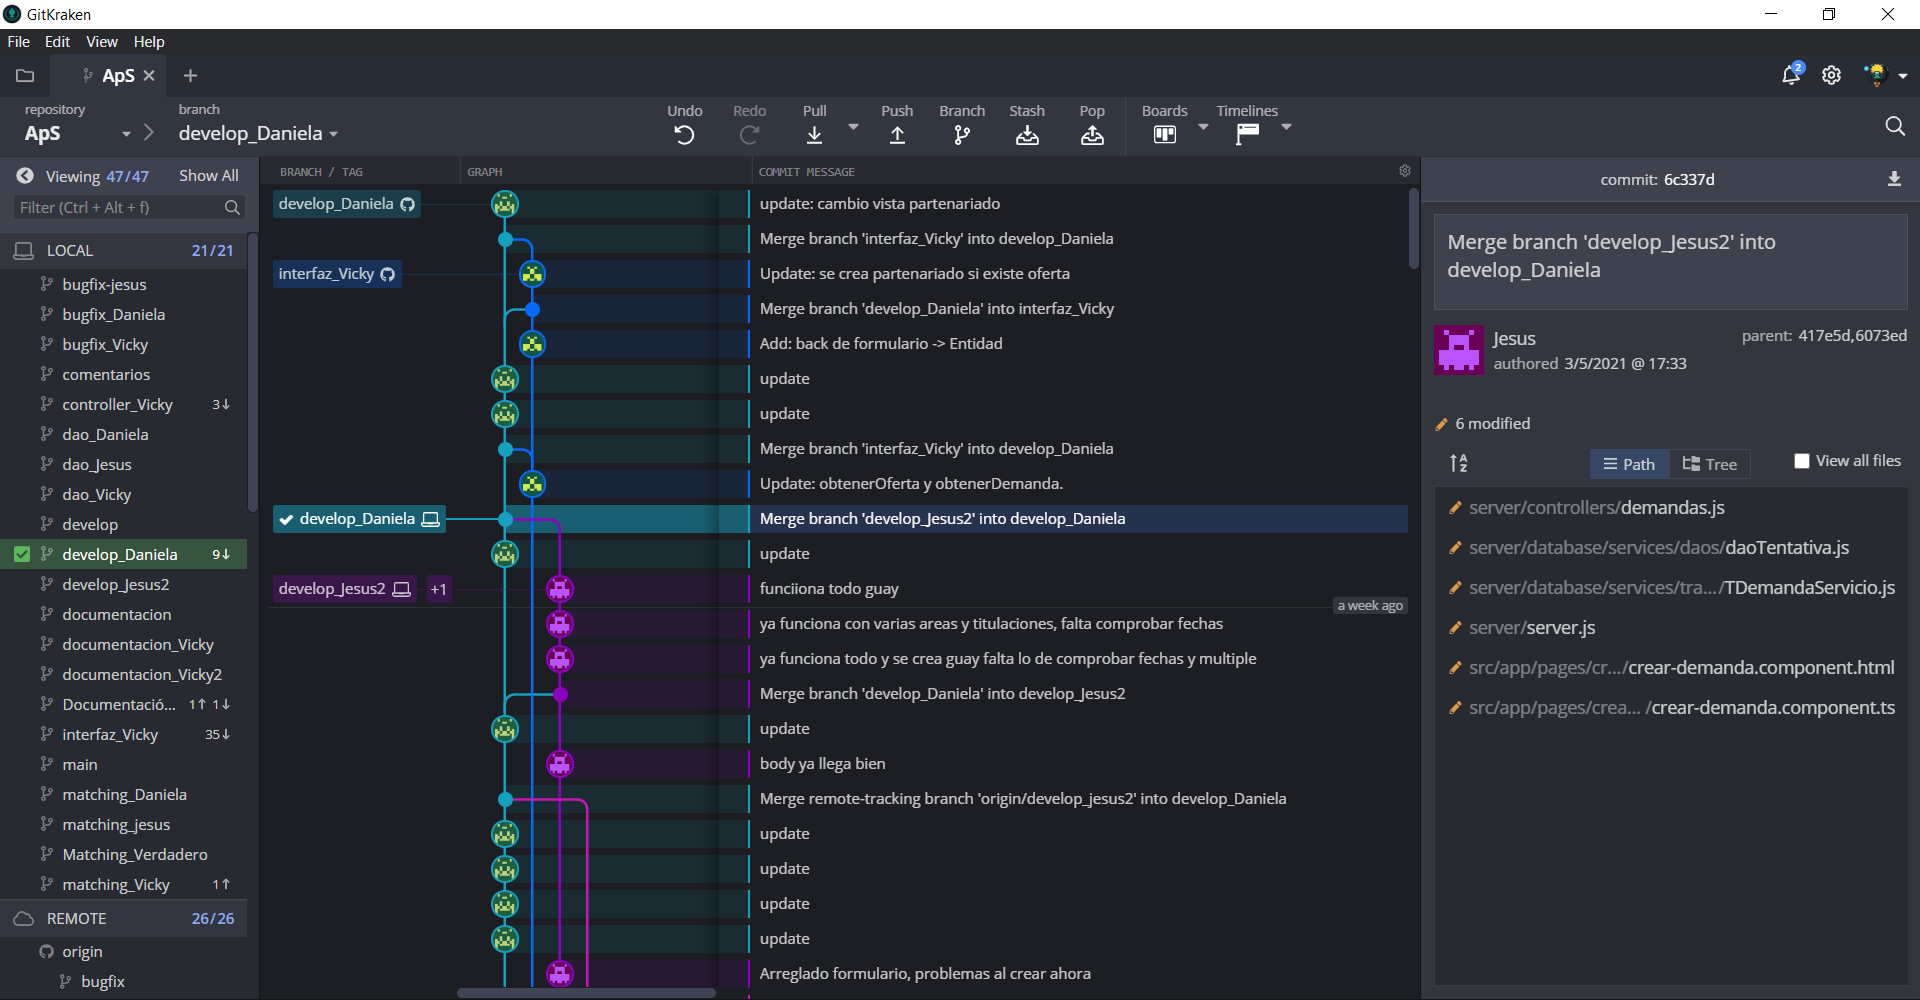
\includegraphics[width=\textwidth]{gitkraken}
	
	\item Pivotal tracker: es una herramienta de product-planning y administración de tareas diseñada para equipos de desarrollo que siguen metodologías de diseño ágiles.
	Esta herramienta permite crear historias de usuario y asignarles una puntuación del 1 al 5 indicando su dificultad y/o tiempo invertido en dichas tareas. Además permite cambiar el estado de las tareas(empezado, finalizado, en revisión...) y cualquier cambio en el estado de dichas tareas se informa por correo de manera automática a quien esté involucrado en ella.
	También permite ver las tareas completadas y rechazadas y generar gráficos indicando el esfuerzo realizado. Esta tecnología fue sugerida por Victoria y nos ha facilitado mucho tanto la organización como el seguimiento de nuestros avances.

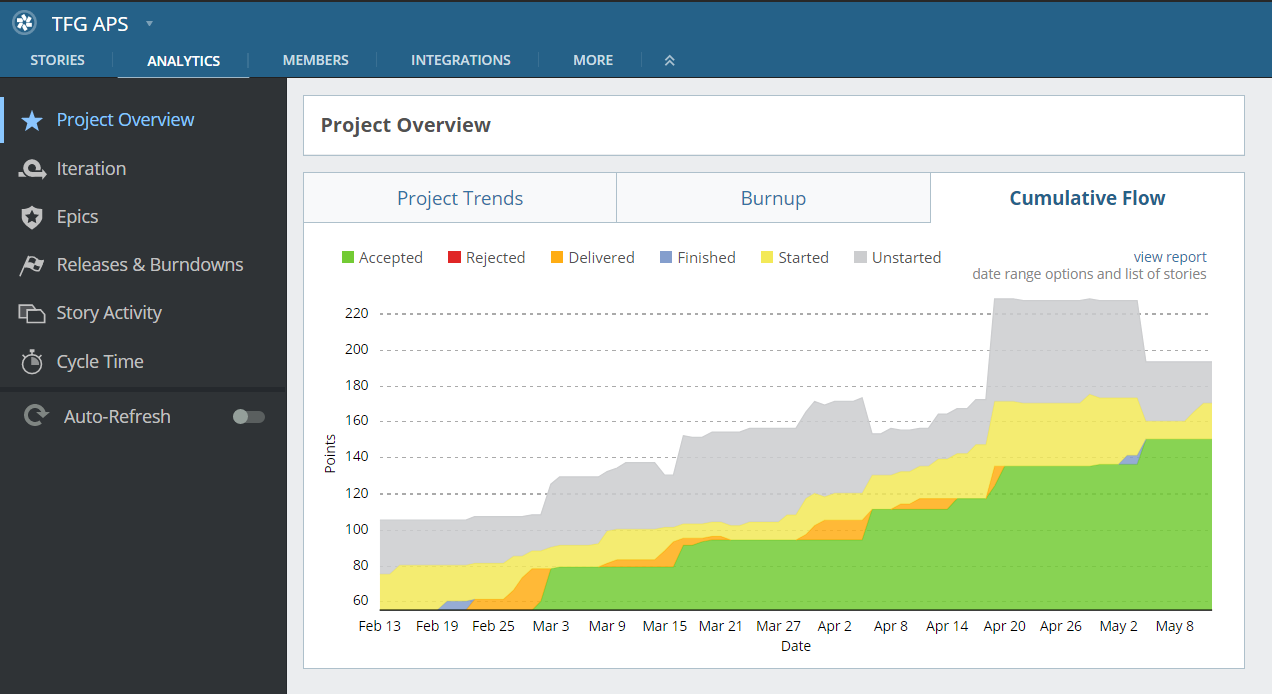
\includegraphics[width=\textwidth]{pivotal}
	
	
	\item LaTex: Es un lenguaje de maquetado utilizado comúnmente en el mundo académico, que es una de las principales razones por la que lo hemos escogido para redactar nuestra memoria, a pesar de que ningún integrante del grupo tuviera experiencia previa con ello. A diferencia de otros procesadores de texto, como Microsoft Word o LibreOffice Writer, se escribe el texto plano y se formatea dicho texto con etiquetas. 
	
	\item MySQL: Aunque nuestro proyecto continúa el trabajo realizado por David Jiménez del Rey y ya contaba con un sistema gestor de bases de datos, dicho sistema era MongoDB y como los datos que se iban a manejar en la aplicación eran en su mayoría relacionales se tomó la decisión de utilizar MySQL para la base de datos. Dado que todos los componentes del grupo tenían experiencia previa en bases de datos sql fue un cambio bien recibido.
	
	\item Modelio: Es un entorno de modelado open-source el cual permite trabajar con un amplio rango de modelos y diagramas. Dado que ya se contaba con experiencia previa en esta herramienta por parte de todos los miembros del equipo, se ha escogido para realizar los modelos de datos necesarios para la aplicación.
	
	\item MySQL Workbench: Es una herramienta para diseño, desarrollo y administración de bases de datos relacionales. 
	Cuenta con funcionalidades de validación de esquemas y modelos promueve las mejores prácticas de los estándares de modelado de datos. También promueve los estándares de diseño específicos de MySQL para evitar errores al generar esquemas relacionales o creando bases de datos MySQL. Por estos motivos junto con su relativa simplicidad es por lo que se ha elegido esta herramienta para hacer los diagramas de entidad-relacion
	
	\item Diagrams.net: Es una herramienta de diseño de diagramas de varios tipos entre los cuales se encuentran diagramas de clases, de flujos, de entidades...
	Es una herramienta muy poderosa pero dado que ningún componente del grupo tenía experiencia previa con ella y para lo único que se necesitaba era para hacer el diagrama de entidad-relación, se descartó el uso de esta aplicación en pos de otra más simple.
	
\end{itemize}
\end{document}
